%%
%% Copyright 2007, 2008, 2009 Elsevier Ltd
%%
%% This file is part of the 'Elsarticle Bundle'.
%% ---------------------------------------------
%%
%% It may be distributed under the conditions of the LaTeX Project Public
%% License, either version 1.2 of this license or (at your option) any
%% later version.  The latest version of this license is in
%%    http://www.latex-project.org/lppl.txt
%% and version 1.2 or later is part of all distributions of LaTeX
%% version 1999/12/01 or later.
%%
%% The list of all files belonging to the 'Elsarticle Bundle' is
%% given in the file `manifest.txt'.
%%

%% Template article for Elsevier's document class `elsarticle'
%% with numbered style bibliographic references
%% SP 2008/03/01

\documentclass[preprint,12pt, a4paper]{elsarticle}

%% Use the option review to obtain double line spacing
%% \documentclass[authoryear,preprint,review,12pt]{elsarticle}

%% For including figures, graphicx.sty has been loaded in
%% elsarticle.cls. If you prefer to use the old commands
%% please give \usepackage{epsfig}

%% The amssymb package provides various useful mathematical symbols
\usepackage{amssymb}
%% The amsthm package provides extended theorem environments
%% \usepackage{amsthm}

%% The lineno packages adds line numbers. Start line numbering with
%% \begin{linenumbers}, end it with \end{linenumbers}. Or switch it on
%% for the whole article with \linenumbers.
\usepackage{lineno}

\usepackage{subfig}
\usepackage{enumitem}
\usepackage{bm}
\usepackage{tikz}
\usetikzlibrary{positioning,shapes,arrows,calc,intersections}

\journal{SoftwareX}

\begin{document}

\begin{frontmatter}

%% Title, authors and addresses

%% use the tnoteref command within \title for footnotes;
%% use the tnotetext command for theassociated footnote;
%% use the fnref command within \author or \address for footnotes;
%% use the fntext command for theassociated footnote;
%% use the corref command within \author for corresponding author footnotes;
%% use the cortext command for theassociated footnote;
%% use the ead command for the email address,
%% and the form \ead[url] for the home page:
%% \title{Title\tnoteref{label1}}
%% \tnotetext[label1]{}
%% \author{Name\corref{cor1}\fnref{label2}}
%% \ead{email address}
%% \ead[url]{home page}
%% \fntext[label2]{}
%% \cortext[cor1]{}
%% \address{Address\fnref{label3}}
%% \fntext[label3]{}

\title{Splipy: B-Spline and NURBS Modelling in Python}

%% use optional labels to link authors explicitly to addresses:
%% \author[label1,label2]{}
%% \address[label1]{}
%% \address[label2]{}

\author{K.~A.~Johannessen}
\author{E.~Fonn}

\address{SINTEF Digital, PO Box 4760, 7465, Trondheim, Norway\\
         Kjetil.Johannessen@sintef.no \\
         Eivind.Fonn@sintef.no
         }

\begin{abstract}
%% Text of abstract (Ca 100 words)
Splipy is a pure python library for the creation, evaluation and manipulation of B-spline and NURBS geometries.
It supports $n$-variate splines of any dimension, but emphasis is made on the use of curves, surfaces and volumes.
The library is designed primarily for analysis use, and therefore allows fine-grained control over many aspects which is not possible to achieve with conventional CAD tools.

\end{abstract}

\begin{keyword}
%% keywords here, in the form: keyword \sep keyword
NURBS \sep B-splines \sep CAD \sep Interpolation \sep Approximation

%% PACS codes here, in the form: \PACS code \sep code

%% MSC codes here, in the form: \MSC code \sep code
%% or \MSC[2008] code \sep code (2000 is the default)

\end{keyword}

\end{frontmatter}

\linenumbers

%% main text

\section{Motivation and significance}
\label{sec:motivation}

Non-uniform rational B-splines (NURBS) have been a staple technology in \emph{computer aided design} (CAD) for many decades.
Their mathematical precision allows the user to create smooth parametric descriptions of curves and surfaces, which is necessary in many engineering applications.
Recent years has seen an increased interest in the use of B-splines and NURBS directly in high-fidelity physics simulations such as the finite element method, thereby uniting geometric modelling and analysis.
The groundbreaking work for these methods, termed \emph{isogeometric analysis} (IGA) can be found in \cite{hughes2005iac}.
While commercial CAD tools do well to facilitate NURBS-based modelling, IGA requires finer control of discretization details, and these are often hidden from the user.
We propose Splipy as a modern easy-to-use Python library that will allow scientist and engineers the detailed control that they need to not only make B-spline meshes that are optimized for analysis, but also work well for modelling.

The software allows for rapid generation of high-quality meshes that can be used directly in IGA programs.
While Splipy offers everything needed in terms of basis function evaluations, derivatives etc.~to build a stand-alone finite element solver, we envision that most users will be content to generate the geometry in Splipy followed by exporting to external solvers.

% \begin{itemize}
%   \item Introduce the scientific background and the motivation for developing the software.
%   \item Explain why the software is important, and describe the exact (scientific) problem(s) it solves.
%   \item Indicate in what way the software has contributed (or how it will contribute in the future) to the process of scientific discovery; if available, this is to be supported by citing a research paper using the software.
%   \item Provide a description of the experimental setting (how does the user use the software?).
%   \item Introduce related work in literature (cite or list algorithms used, other software etc.).
% \end{itemize}

\section{Software description}
\label{sec:description}

The core tenet of Splipy is the manipulation of \emph{spline objects}, by which is meant a mapping from a $n$-dimensional \emph{parameter space},
\begin{equation}
  \label{eqn:paramspace}
  \mathcal{P} = [l_1, r_1] \times [l_2, r_2] \times \cdots \times [l_n, r_n]
\end{equation}
into \emph{physical space} $\mathbb{R}^d$.
Conventionally, $d \geq n$.
In spline terms, each parameter interval $[l_i, r_i]$ is subdivided into a \emph{knot vector}
\begin{equation}
  \label{eqn:knotvector}
  l_i = k_0 \leq k_1 \leq k_2 \leq \cdots \leq k_{n_i} = r_i,
\end{equation}
with nondecreasing \emph{knots} $k_j$.
Given a knot vector and a polynomial degree $p_i$, there is a unique B-spline basis $B_j(x_i)$ defined on the interval $[l_i, r_i]$.
Each basis function $B_j$ is piecewise polynomial with degree $p_i$ in all knot intervals $[k_m, k_{m+1}]$, and is supported on exactly $p_i+1$ such intervals.

Given a choice of knot vector and degree for each direction $i=1,\ldots,n$, the full B-spline basis is defined on $\mathcal{P}$ as
\begin{equation}
  \label{eqn:bspline-multi}
  B_{j_1,\ldots,j_n}(x_1,\ldots,x_n) = B_{j_1}(x_1) \cdots B_{j_n}(x_n)
\end{equation}
and a \emph{spline object} is nothing more than a function in the span of this basis, i.e.~a function $s: \mathcal{P} \to \mathbb{R}^d$ such that
\begin{equation}
  \label{eqn:splineobj}
  s(\bm x) = \sum_{j_1, \ldots, j_n} \bm c_{j_1, \ldots, j_n} B_{j_1, \ldots, j_n}(\bm x).
\end{equation}
Here, the coefficients $\bm c_{j_1, \ldots, j_n} \in \mathbb{R}^d$ are termed \emph{control points}.

Splipy is concerned with the creation and manipulation of these mappings and the objects they represent (that is, the image of $\mathcal{P}$ by $s$ in $\mathbb{R}^d$).
With the intended emphasize on analysis: fine control over both the knot vectors and control points are provided.
These quantities dictates the properties of the parametric representation and the geometric mapping respectively.

\subsection{Software Architecture}
\label{sec:architecture}

There are three main classes which are exposed to the user: \texttt{Curve}, \texttt{Surface} and \texttt{Volume}.
All inherit from the \texttt{SplineObject} superclass, which contains common methods such as affine transformations, evaluation and get methods.
See Figure~\ref{fig:hierarchy}.
It is possible to create such spline objects manually, by specifying knot vectors and control points, however most users will be using a wide range of ``factory'' functions.
These can be found in the submodules \texttt{curve\_factory}, \texttt{surface\_factory} and \texttt{volume\_factory}.
More advanced geometries can then be created by using the rich interface for manipulating spline objects.
Generally Splipy scripts follow a bottom-up construction scheme where curves are created from points, surfaces are created from curves and finally volumes are created from the surfaces.

\begin{figure}
  \begin{center}
    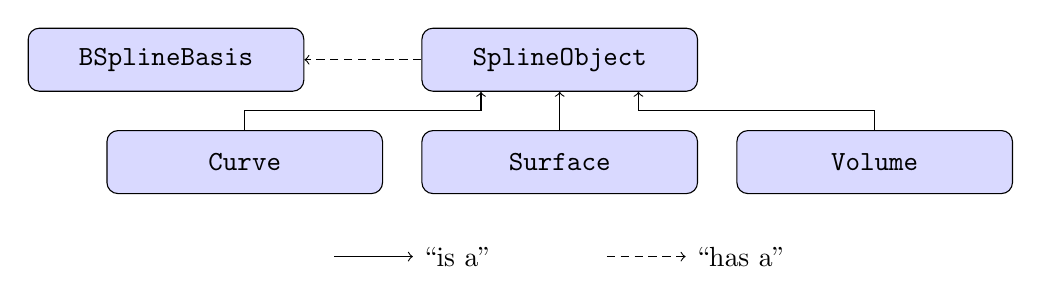
\begin{tikzpicture}[
      class/.style={rectangle, draw=black, fill=blue!15, align=center, rounded corners, minimum width=3.5cm, minimum height=0.8cm},
      ]
      \node[class] (BS) at (-5.0,0) {\texttt{BSplineBasis}};
      \node[class] (SO) at (0,0) {\texttt{SplineObject}};
      \node[class] (CU) at (-4.0,-1.3) {\texttt{Curve}};
      \node[class] (SF) at (0,-1.3) {\texttt{Surface}};
      \node[class] (VO) at (4.0,-1.3) {\texttt{Volume}};

      \draw[->] (SF.north) -- (SO.south);
      \draw[->] (CU.north) -- ++(0,0.25) -| ([xshift=-1cm]SO.south);
      \draw[->] (VO.north) -- ++(0,0.25) -| ([xshift=1cm]SO.south);
      \draw[->, densely dashed] (SO.west) -- (BS.east);

      \node (isa) at (-1.3,-2.5) {``is a''};
      \draw[->] ([xshift=-1cm]isa.west) -- (isa.west);

      \node (hasa) at (2.3,-2.5) {``has a''};
      \draw[->, densely dashed] ([xshift=-1cm]hasa.west) -- (hasa.west);
    \end{tikzpicture}
  \end{center}
  \caption{Class hierarchy of Splipy.}
  \label{fig:hierarchy}
\end{figure}

\subsection{Software Functionalities}
\label{sec:functionality}

The library allows for rapid creation of elementary mathematical constructs such as line, circle, disc, sphere, torus, cylinder and teapots.
Some of these have multiple parameterization options, such as disc or sphere, see section~\ref{sec:sphere}.

The factory classes also contain spline-related constructors, such as \\
\textbf{Curve Factories}
\begin{itemize}
    \setlength\itemsep{-.5em}
    \item Bezier curves
    \item Hermite Interpolation
    \item Cubic Curve Interpolation
    \item B-spline Interpolation
    \item Least Square Fit
    \item Adaptive Curve Fit
\end{itemize}
\textbf{Surface Factories}
\begin{itemize}
    \setlength\itemsep{-.5em}
    \item Sweep
    \item Revolve
    \item Loft
    \item Extrude
    \item Interpolation
    \item Least Square Fit
    \item Edge Curves (interior from four edges)
\end{itemize}
\textbf{Volume factories}
\begin{itemize}
    \setlength\itemsep{-.5em}
    \item Revolve
    \item Extrude
    \item Loft
    \item Interpolation
    \item Least Square Fit
\end{itemize}

\begin{figure}
  \begin{center}
    \subfloat[\textbf{Sweep:} dragging one curve along another]{
      \label{fig:sweep}
      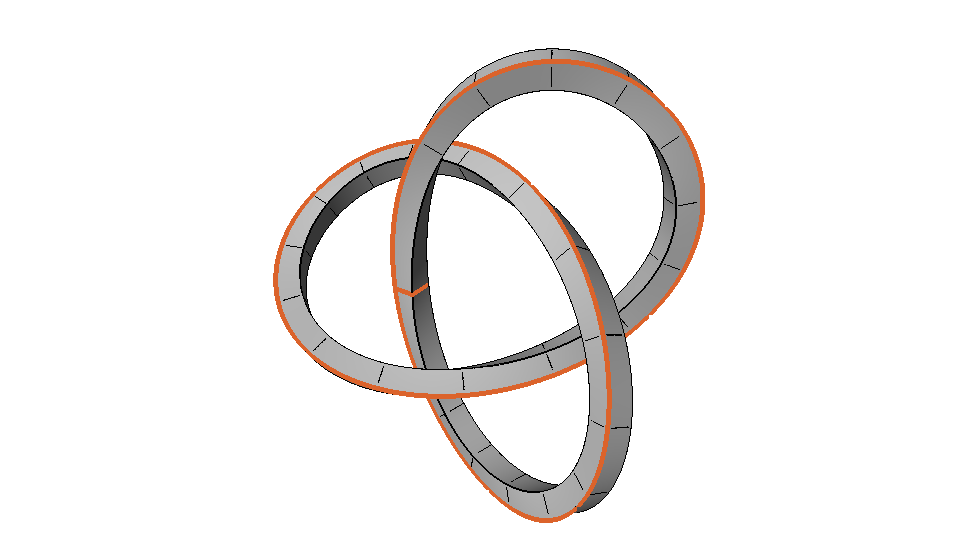
\includegraphics[height=.28\textwidth]{figs/sweep}
    }
    \hspace{.02\linewidth}
    \subfloat[\textbf{Revolve:} rotating a curve around an axis]{
      \label{fig:revolve}
      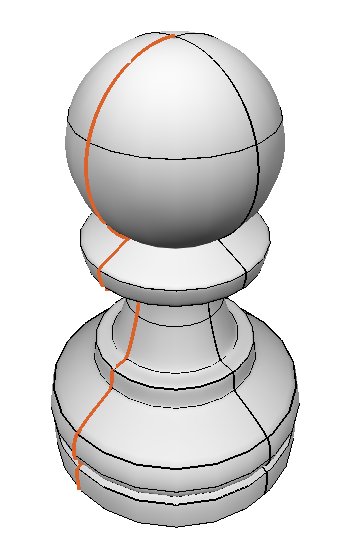
\includegraphics[height=.28\textwidth]{figs/revolve}
    }
    \hspace{.02\linewidth}
    \subfloat[\textbf{Loft:} interpolates a given set of curves]{
      \label{fig:loft}
      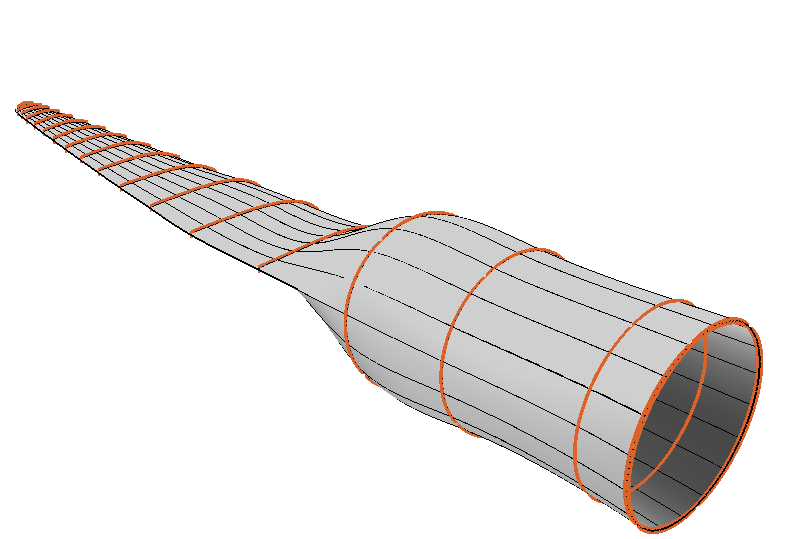
\includegraphics[height=.28\textwidth]{figs/loft2}
    }
    \caption{\textbf{surface\_factory:} Splipy follows a bottom-up design principle where surfaces typically are constructed from defining curves}
  \end{center}
\end{figure}

% \begin{figure}
%   \begin{center}
%     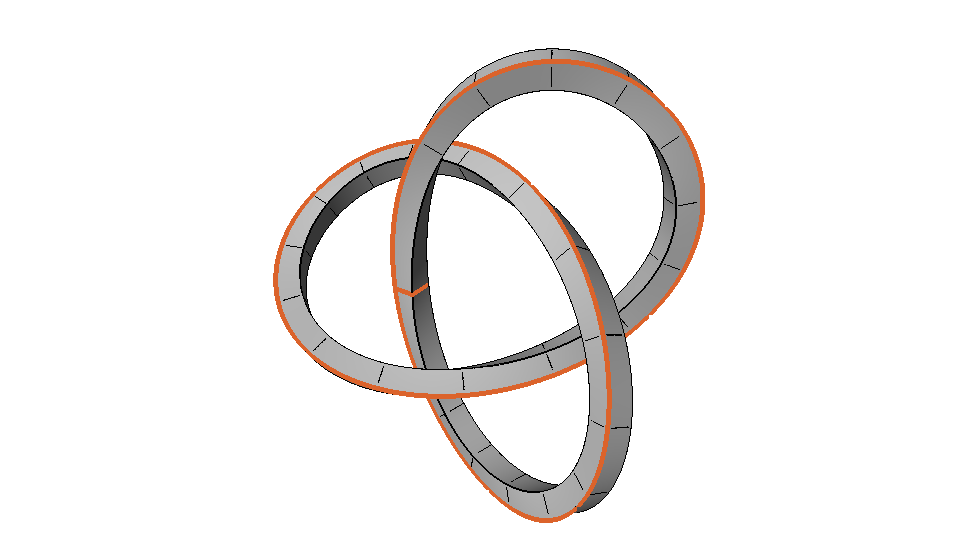
\includegraphics[width=.4\textwidth]{figs/sweep}
%     \caption{\textbf{Sweep:} create a surface by dragging one curve along another}
%     \label{fig:loft}
%   \end{center}
% \end{figure}
% \begin{figure}
%   \begin{center}
%     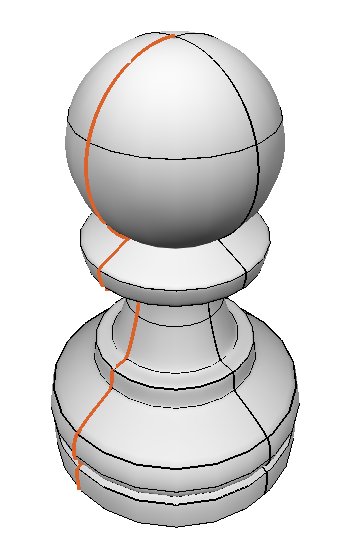
\includegraphics[width=.4\textwidth]{figs/revolve}
%     \caption{\textbf{Revolve:} create a surface by rotating a curve around an axis}
%     \label{fig:loft}
%   \end{center}
% \end{figure}

We now elaborate on a few selected functions.

\subsubsection{Adaptive Curve fitting}
\label{sec:adaptive-curve-fit}
For parametric representation of some target curve $x(t)$ we provide a \texttt{fit} function in \texttt{curve\_factory} which employs a posteriori error estimation to provide a best fit $x_h(t)$ to the curve.
It is a four-stage iterative algorithm which works as follows:
Start with a uniform knot vector; for the current release this knot vector is cubic and contains 10  basis functions.
\\ \textbf{step 1:}
Compute the Greville abscisscae $t^*_i = \sum_{j=i}^{i+p} k_j$ and interpolate on these points $x(t_i^*) = x_h(t_i^*)$.
\\ \textbf{step 2:}
Compute the error $\|x(t)-x_h(t)\|_{L^2(k_i,k_{i+1})}$ for all knot spans $(k_i,k_{i+1})$
\\ \textbf{step 3:}
For all knot spans $(k_i,k_{i+1})$, compute the expected error $\varepsilon_i$ and interpolation error $\varepsilon_{h,i}$ defined as
\begin{eqnarray}
    \varepsilon_i     & = & \frac{k_{i+1} - k_i}{k_n - k_0}\varepsilon \\
    \varepsilon_{h,i} & = & \int_{k_i}^{k_{i+1}} x(t) - x_h(t)\quad dt
\end{eqnarray}
where $\varepsilon$ is some user-defined global tolerance
\\ \textbf{step 4:}
Since we know that our approximation \cite{deboor1978apg} to converge wrt the knot span size $h=k_{i+1}-k_i$ as $\|x(t)-x_h(t)\|_{L^2} = \mathcal{O}(h^{p+1})$ with $p$ our spline degree, we expect that inserting
\begin{equation}
    n = 2^{-(p+1)}\frac{\varepsilon_{h,i}}{\varepsilon_i}
\end{equation}
new knots will give us the target error.
These knots are then inserted into their relevant knot span and a new interpolation is computed.

These iterations are carried out until the global tolerance is achieved.

\subsubsection{Interior from edges}
\label{sec:interior-from-edges}
The default method to produce the interior mesh from 4 edge curves is an algorithm known as Coons Patch \cite{coons1967sfc}. The logic on this is the following. Assume that you have a parameterized left and right curve given as $c_1(v)$ and $c_2(v)$ as well as a bottom and top curve $c_3(u)$ and $c_4(u)$, and without loss of generality assume $u,v\in[0,1]$. By creating 3 different surfaces $S_1(u,v)$, $S_2(u,v)$ and $S_3(u,v)$ which interpolate the left/right curves, top/bottom curves and the four corners respectively
\begin{eqnarray*}
    S_1(u,v) & = & (1-u)c_1(v) + uc_2(v) \\
    S_2(u,v) & = & (1-v)c_3(u) + vc_4(u) \\
    S_3(u,v) & = & (1-u)(1-v)c_1(0) + u(1-v)c_2(0) + (u-1)vc_4(0) + uvc_4(1) \\
\end{eqnarray*}
then the following surface will interpolate all edges simultaneously:
\begin{equation}
    S(u,v)   = S_1(u,v) + S_2(u,v) - S_3(u,v)
\end{equation}

While coons patch is incredible versatile it is not general enough that it will work on all cases.
For harder input curves the resulting surface $S(u,v)$ might be self-intersecting and contain folds.
For a more robust method it is possible to formulate the parametrization problem as Poisson problem or elasticity problem (linear or finite strain).
or the Poisson case this is done by setting up the following partial differential equation:
\begin{equation}
    \begin{array}{rcll}
    \frac{\partial^2 x}{\partial u^2} + \frac{\partial^2 x}{\partial u^2} & = & 0 &, u,v\in [0,1] \\
    x(0,v) & = & c_1(u) &, v = 0 \\
    x(1,v) & = & c_2(u) &, v = 1 \\
    x(u,0) & = & c_3(v) &, u = 0 \\
    x(u,1) & = & c_4(v) &, u = 1
    \end{array}
\end{equation}
and then solving for $x$, typically through some numerical scheme such as the finite element method.
In Splipy this is done by the use of the Nutils library \cite{van_zwieten2018n} and is provided as an optional dependency.
To complete the parametrization you would have to solve for both the parametrization of $y$ in addition to the one for $x$.

For details on both the Poisson and the elasticity implementation see the work of Hansvold \cite{hansvold2015mgt}. 


\subsubsection{Sphere parametrization}
\label{sec:sphere}
It is well known that perfect circles cannot be represented as B-splines, but can be represented as non-uniform rational B-splines (NURBS).
However, there is multiple ways of parametrizing the circle and its surface and volume equivalent.
In particular, we can do a polar parametrization which would include a geometric singularity point at the origin, or one might do what is dubbed a ``square'' parametrization which computes the interior of the four edge curves given by 4 circle segments.
These can be seen in Figure~\ref{fig:surface-disc} along with a hybrid parametrization which uses 5 different patches.
Note that the square parametrization, have a singular Jacobian at its four corners, where the isocurves in both parametric directions are parallel.
Depending on where you would need optimal parametrization: the origin or the outer boundary, one might chose one or the other parametrization.

\begin{figure}
  \begin{center}
    \subfloat[\textbf{Radial:} or polar parametrization]{
      \label{fig:disc-radial}
      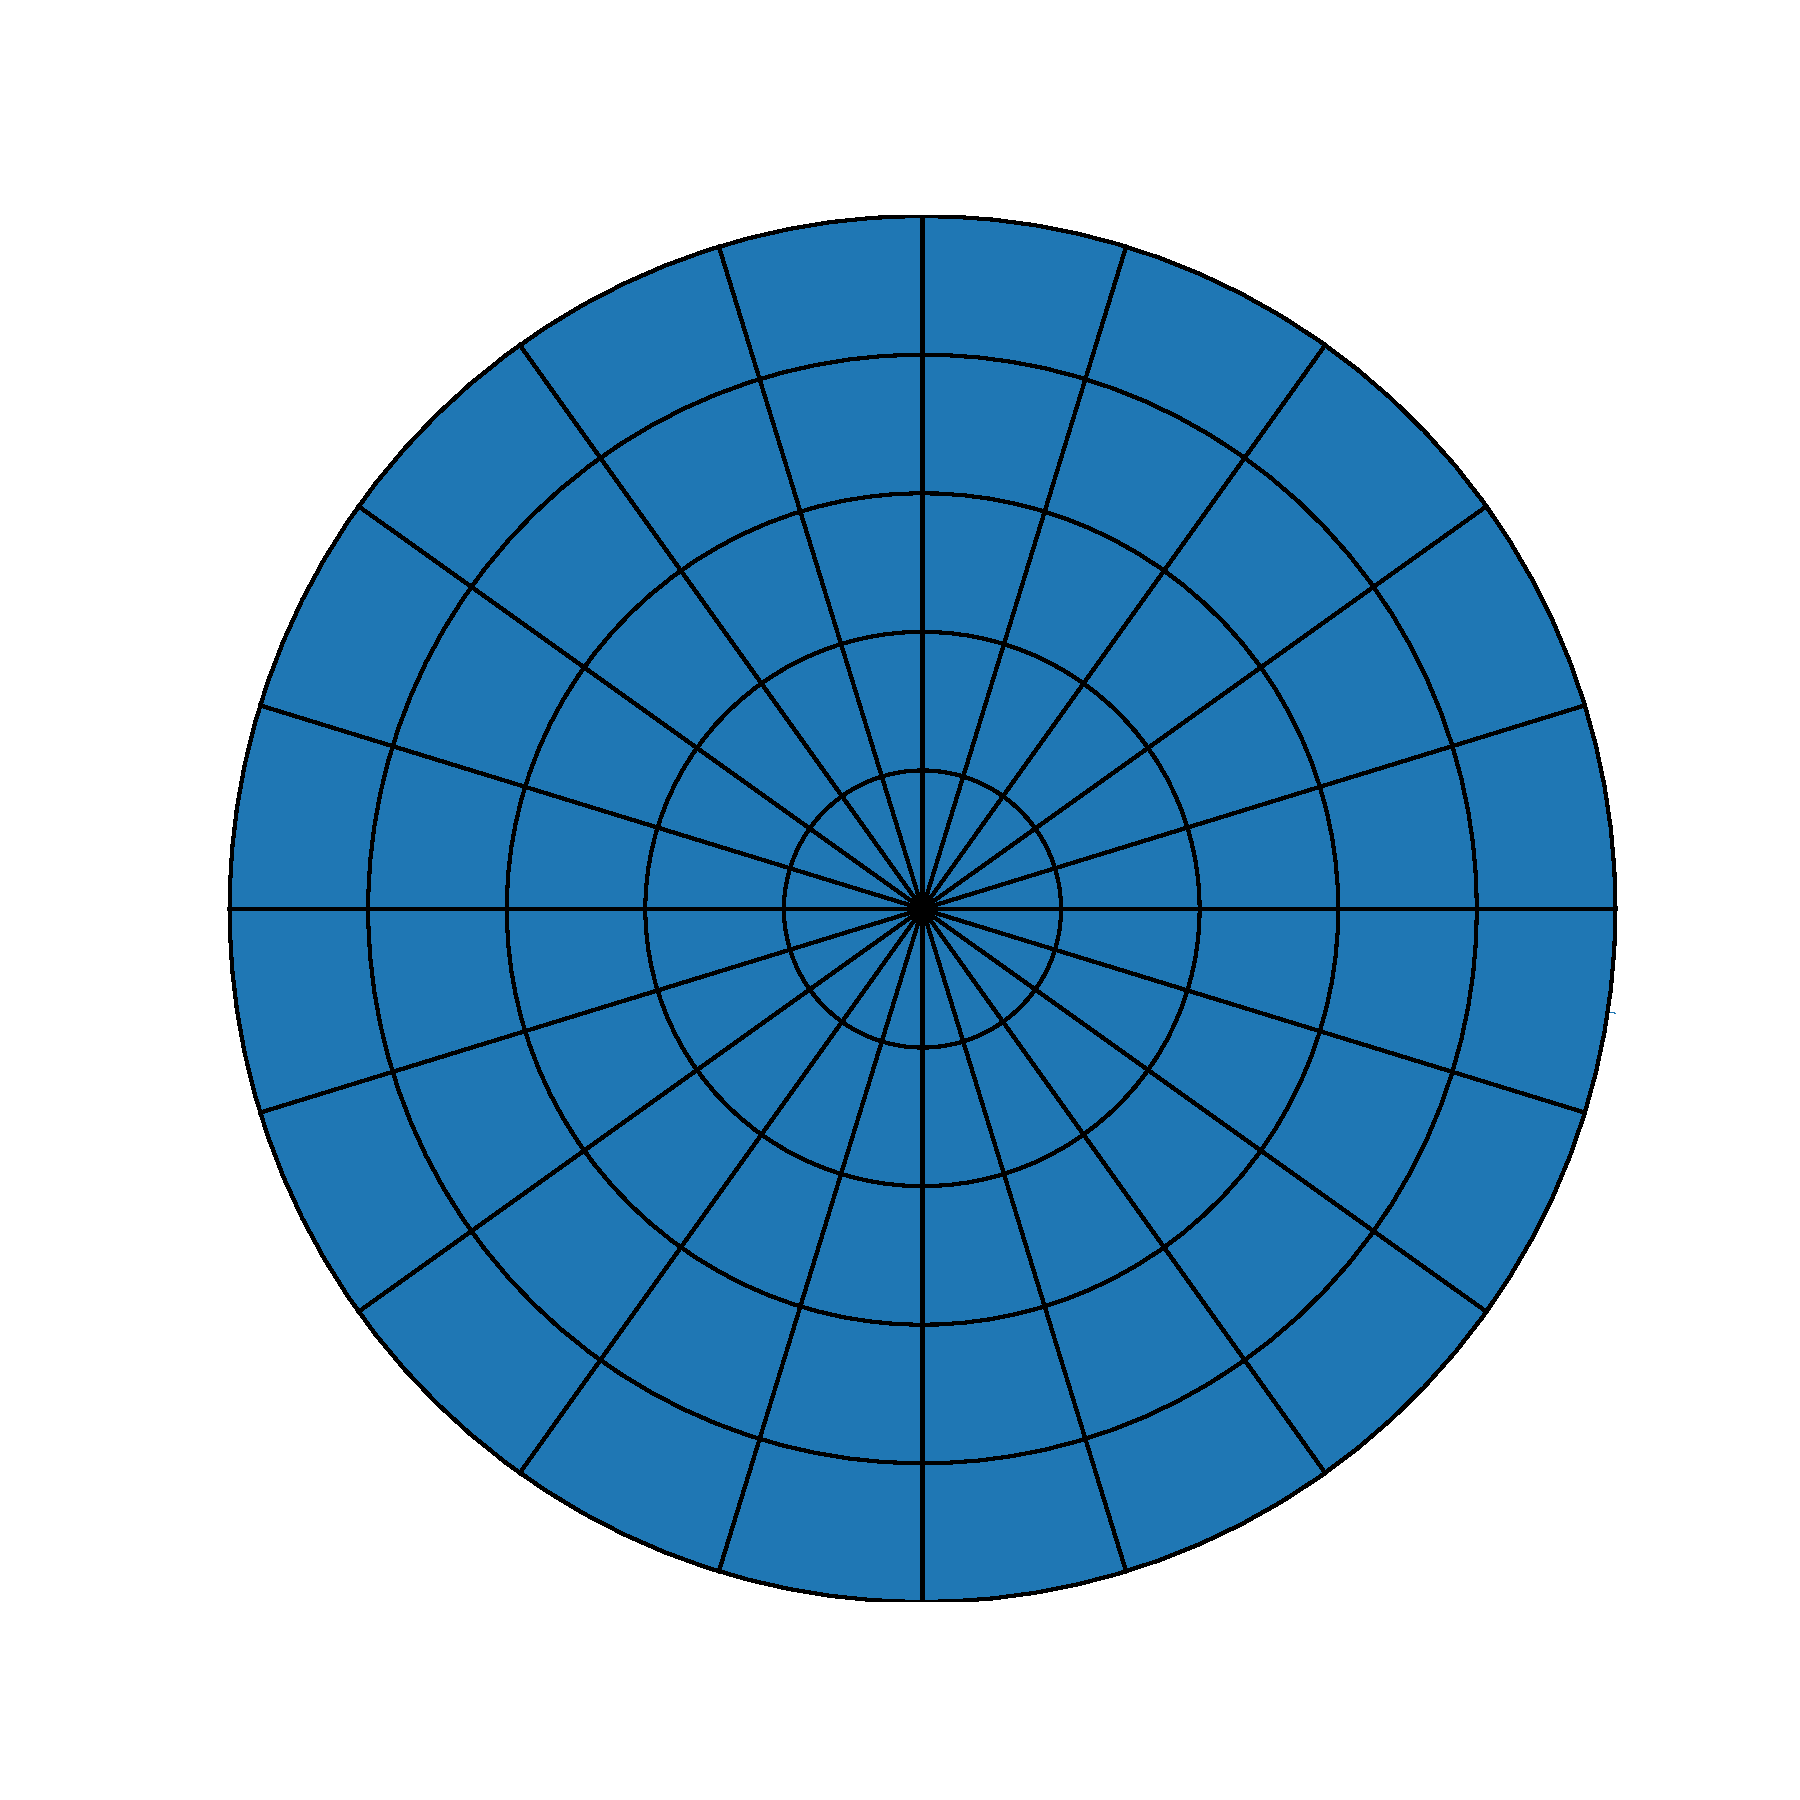
\includegraphics[height=.28\textwidth]{figs/disc-radial}
    }
    \hspace{.02\linewidth}
    \subfloat[\textbf{Square:} parametrization with 4 corners]{
      \label{fig:disc-square}
      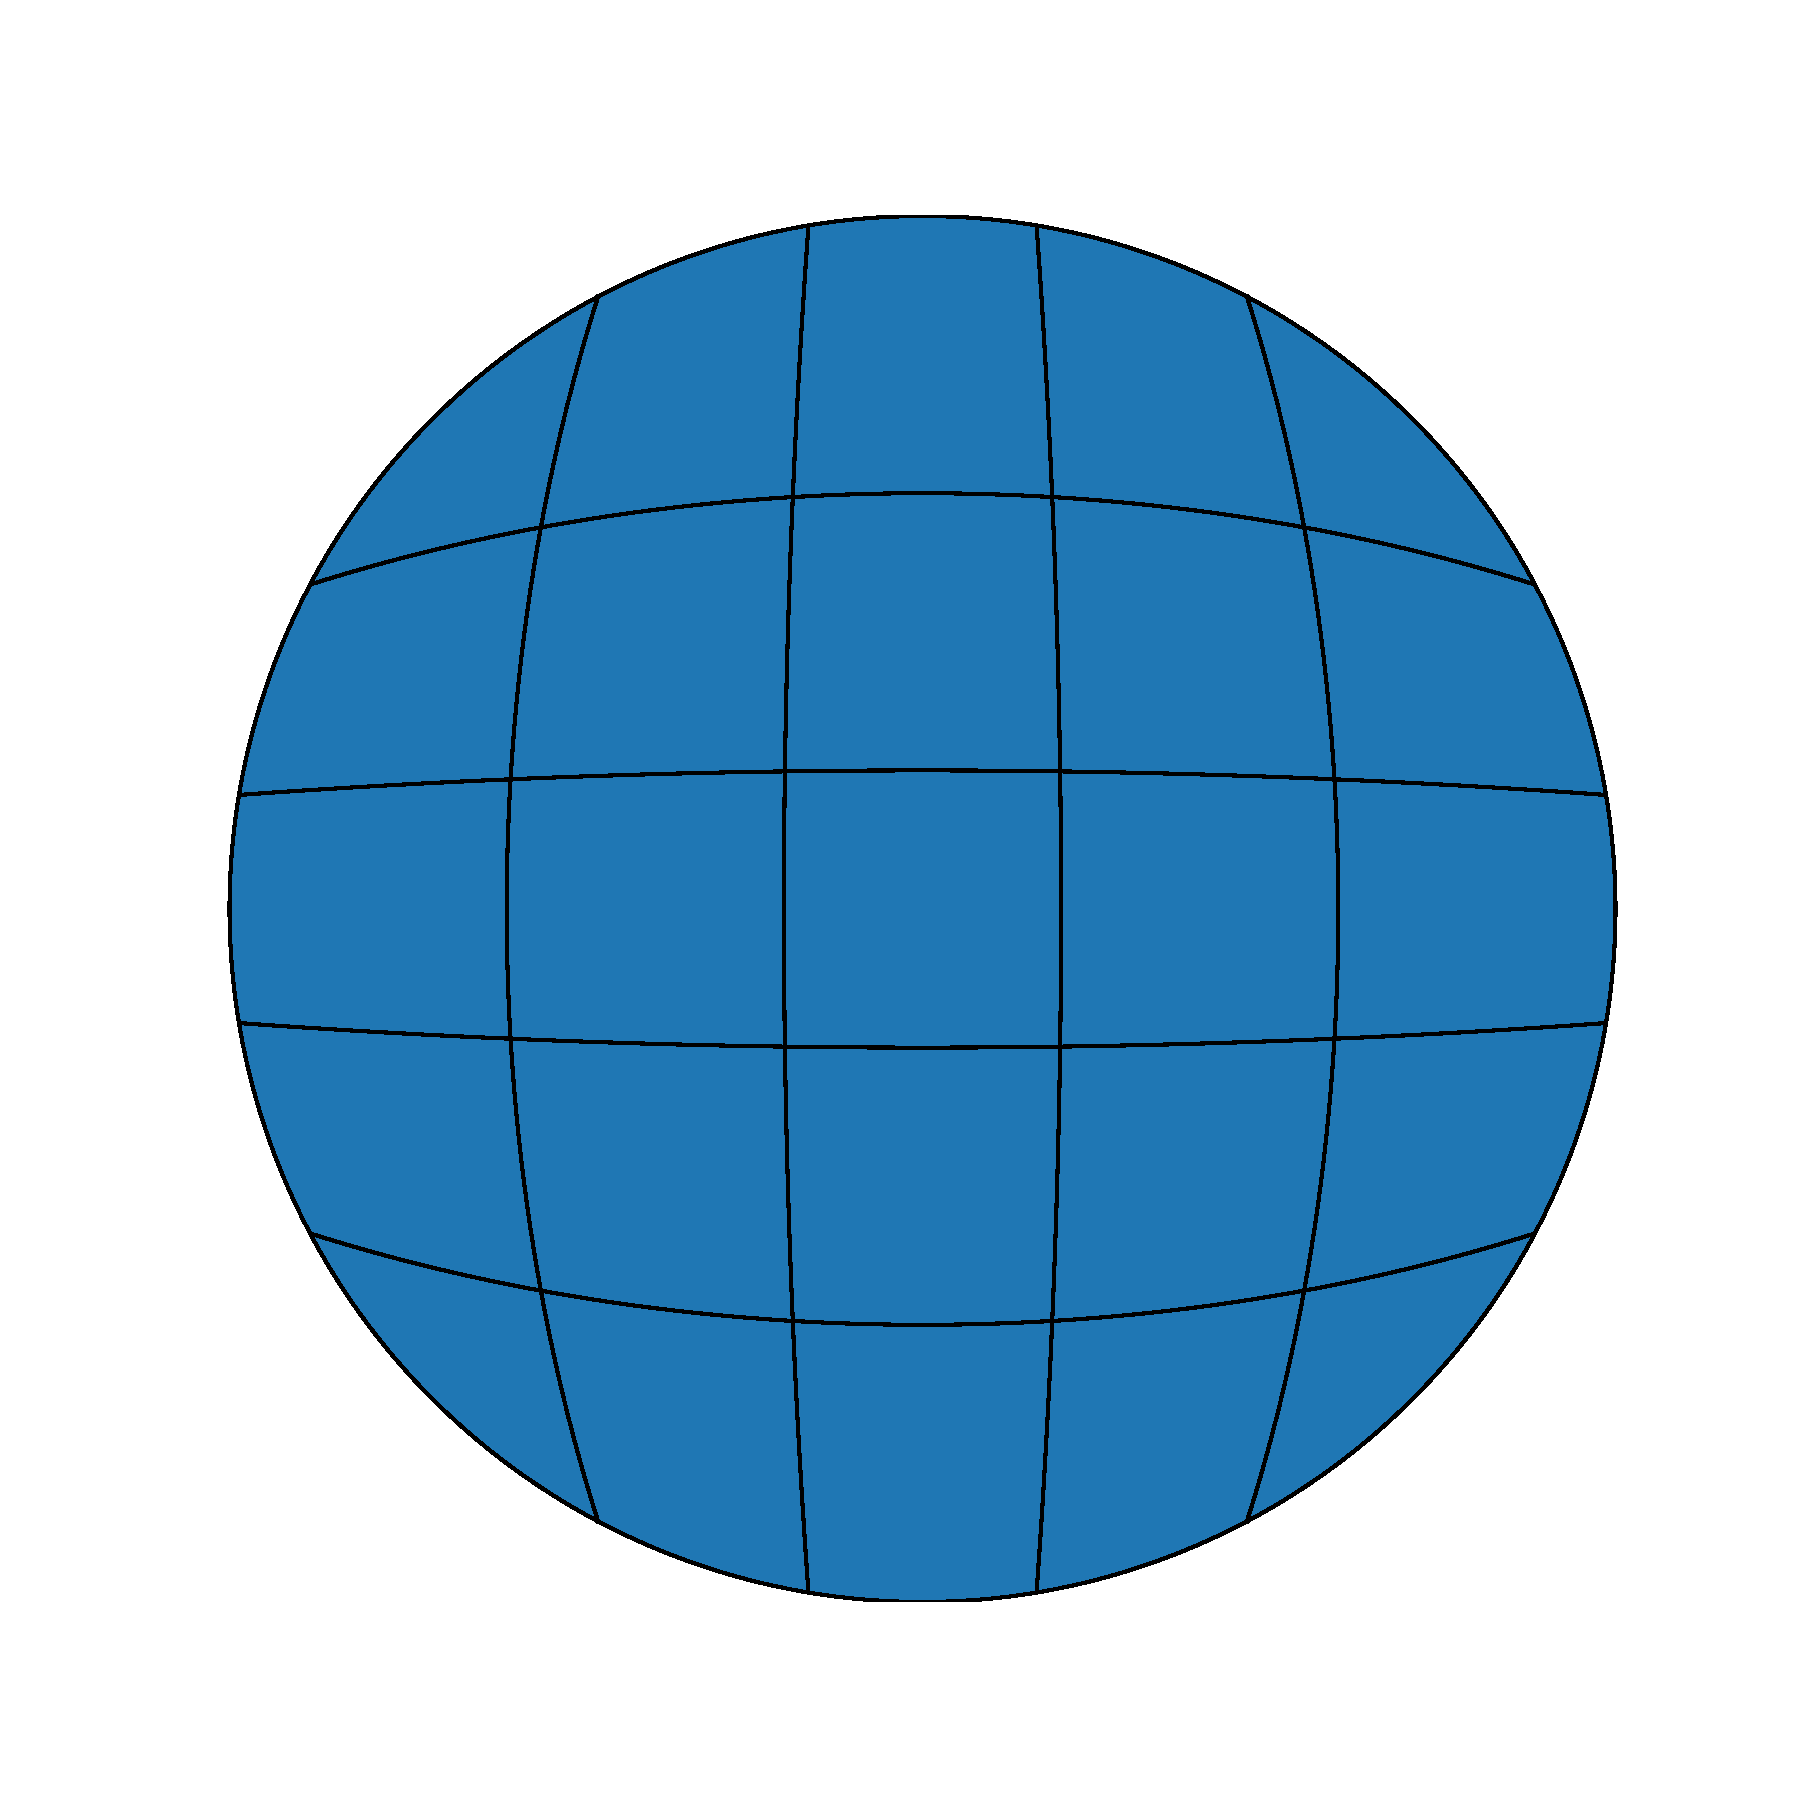
\includegraphics[height=.28\textwidth]{figs/disc-square}
    }
    \hspace{.02\linewidth}
    \subfloat[\textbf{Hybrid:} 5 different patches]{
      \label{fig:disc-5patch}
      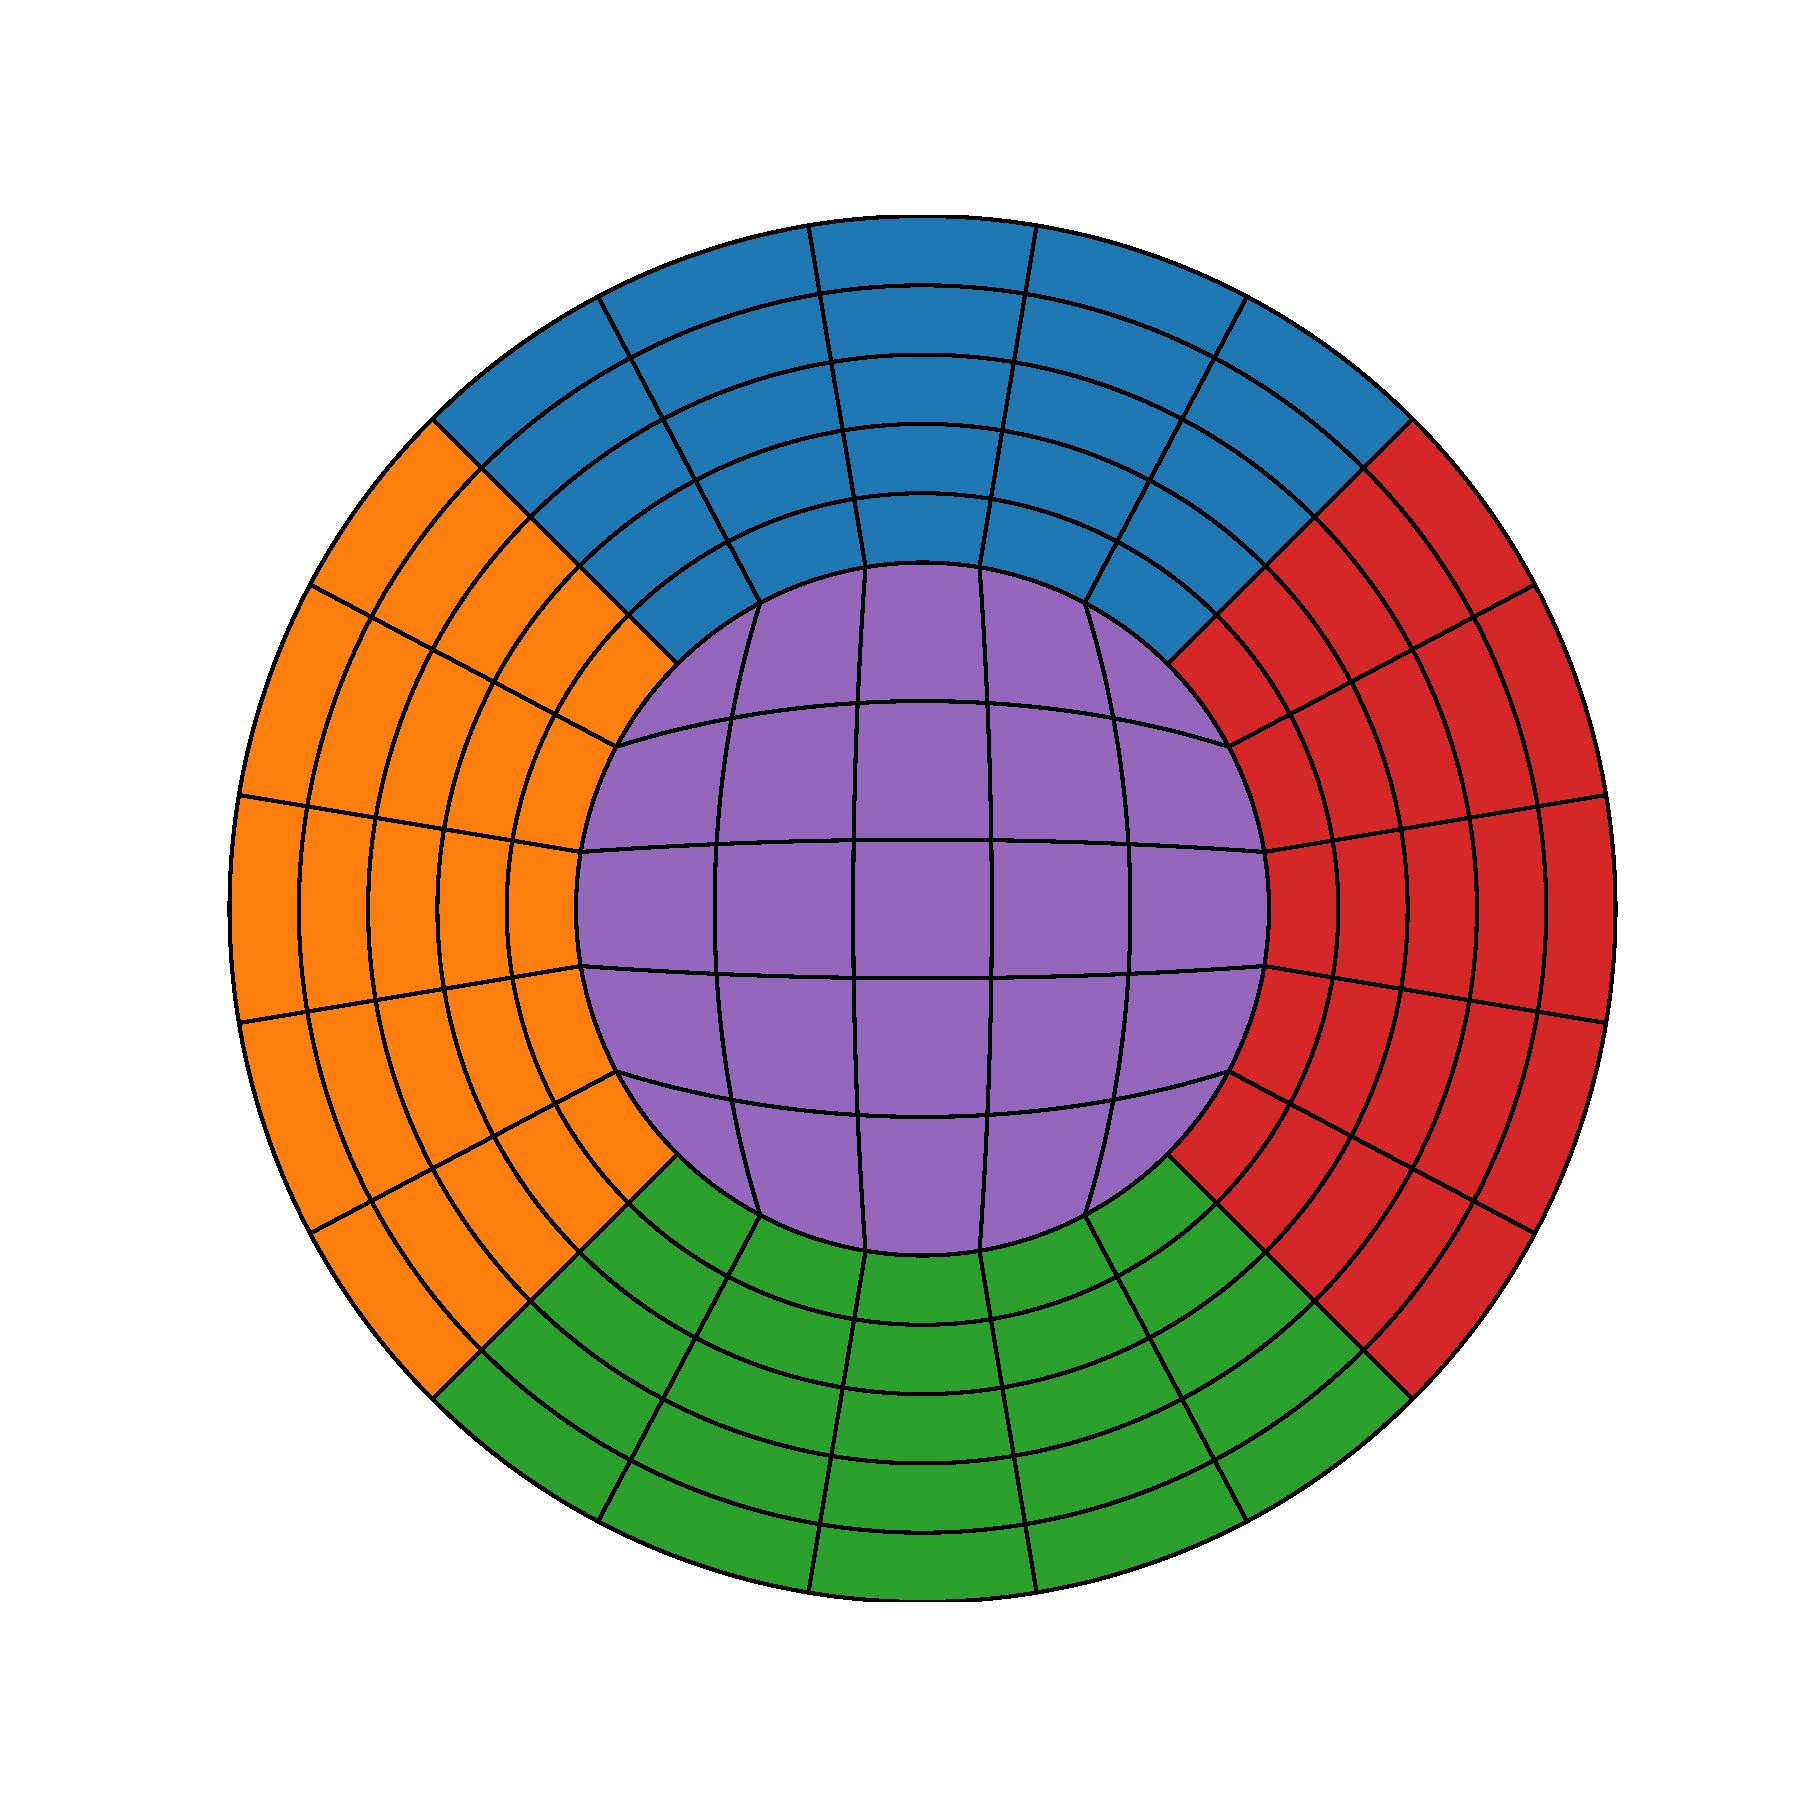
\includegraphics[height=.28\textwidth]{figs/disc-5patch}
    }
    \caption{\textbf{Disc:} multiple discretization options for the same geometry is provided. Here we show three different versions of the disc $\|\mathbf{x}\|^2<1$, each with different benefits. In particular, the vanishing Jacobian can be located at the domain center, boundary or interior respectively, depending on the particular needs of the application.}
    \label{fig:surface-disc}
  \end{center}
\end{figure}

The volumetric parametrization of the sphere, does also have a ``square'' version which avoids the north- and south-pole singularity given by a spherical coordinate parametrization.
For details on the derivation of this particular parametrization, see Cobb \cite{cobb1988tts}.
These are shown in Figure~\ref{fig:volume-disc}

\begin{figure}
  \begin{center}
    \subfloat[\textbf{Radial:} or spherical parametrization]{
      \label{fig:sphere-radial}
      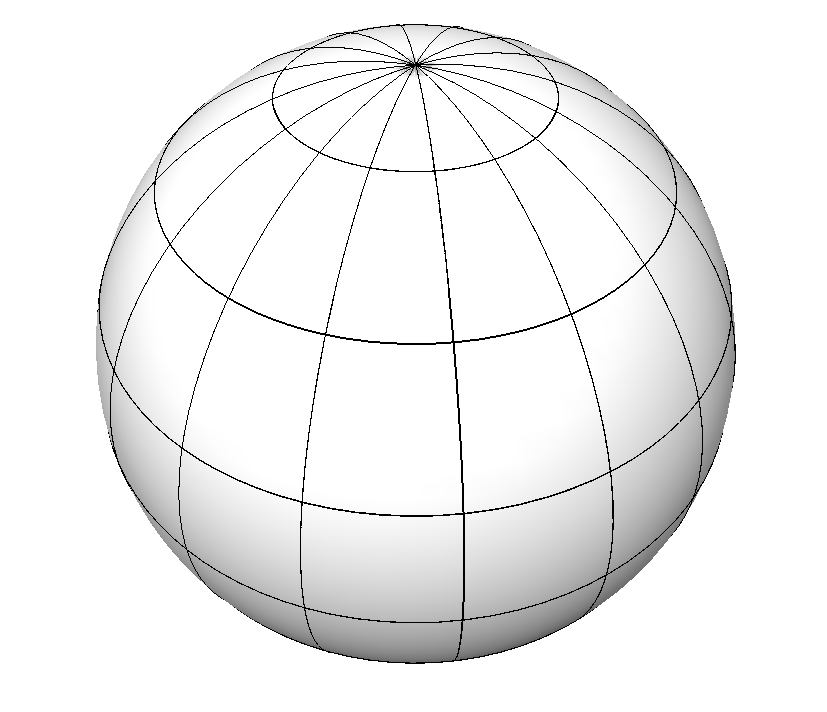
\includegraphics[height=.38\textwidth]{figs/sphere-radial}
    }
    \hspace{.02\linewidth}
    \subfloat[\textbf{Square:} parametrization with 8 corners]{
      \label{fig:sphere-square}
      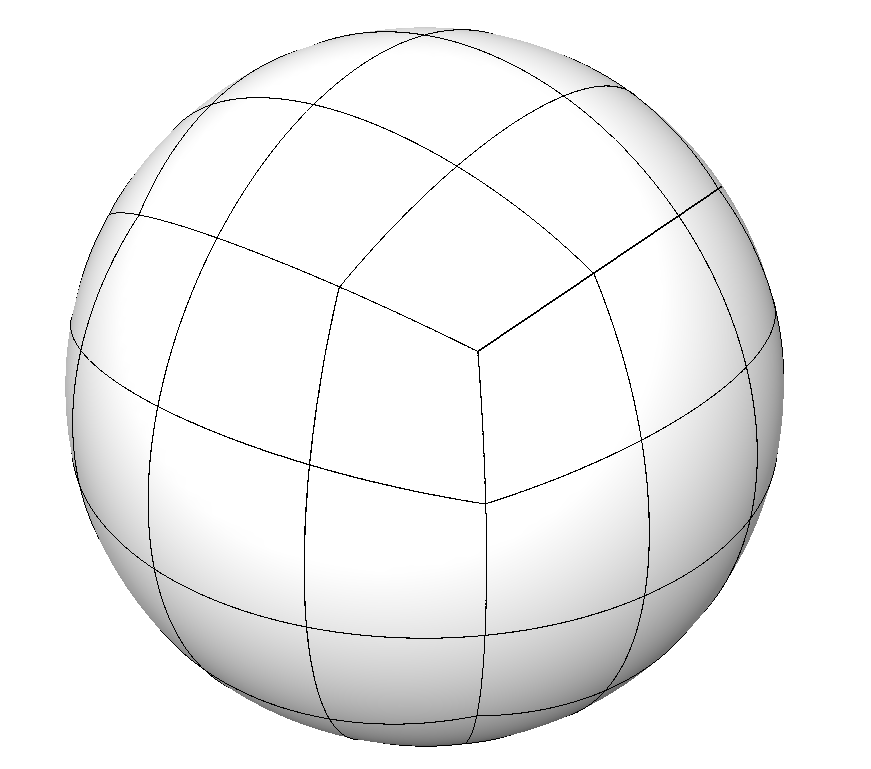
\includegraphics[height=.38\textwidth]{figs/sphere-square}
    }
    \caption{\textbf{Sphere:} multiple discretization options for the same geometry is provided. Here we show two different versions of the unit ball $\|\mathbf{x}\|^2<1$. In particular, the vanishing Jacobian can be located at the domain center or boundary. NURBS representations allow for perfect geometry representation in either case.}
    \label{fig:volume-disc}
  \end{center}
\end{figure}

\subsection{Sample code snippets analysis (optional)}
\label{}

\section{Illustrative Examples}
\label{sec:naca}

The following describes in brief detail the meshing of a NREL 5MW reference wind turbine blade, as described in \cite{Jonkman2009drw}.
This meshing procedure is described in more detail in \cite{Fonn2015sbm} and was performed entirely with Splipy.
This blade is defined as an surface interpolating a number of different airfoils placed at increasing distance from the origin, each of them with a specific shape (e.g.~NACA or DU standard airfoil designs), size and angle of attack.

The construction of the blade itself is relatively straightforward.
Splipy makes possible the description of each defining airfoil as a periodic spline curve with consistent discretization (that is, equal knot vectors).
From this, the entire blade can be lofted in a single operation, see Figure~\ref{fig:airfoils} (left) and \cite{Fonn2015sbm}.
In order to prevent the resulting surface from becoming self-intersecting, an intermediate lower-order interpolation step is inserted.
This strategy is also described in \cite{Fonn2015sbm}.

The objective of the mesh is to perform flow simulations \emph{around} the blade, so it is necessary also to create a volumetric mesh of a suitably large region.
At each designated airfoil, a circular curve is generated at a certain radius, again with a consistent discretization in order to facilitate interpolation.
The surface between the airfoil and the circle is then mapped using a technique known as \emph{orthogonal transfinite interpolation} (OTI), see \cite{Fonn2015sbm} for details.
This technique is intended to ensure that the mesh lines near the airfoil lie orthogonal to the boundary, while the mesh itself remains suitably regular and not self intersecting.
To ensure this, OTI uses an iterative process, generating the enveloping curve one mesh line at a time from the interior toward the exterior.
At each step, the enveloping curve is defined as a weighted mean between two curves: a standard linear interpolation between the \emph{previous} enveloping curve and the exterior circle, and the orthogonal outward projection of the previous enveloping curve by a suitable distance.
The weight of this mean is chosen so that the orthogonal projection dominates near the airfoil, while the linear interpolation dominates further away.
In addition to this, each enveloping curve is further smoothed by a Laplacian operator, further reducing the risk of self intersections.
Each enveloping curve thus defined, the region between the airfoil and the circle can be meshed by lofting, and the volumetric mesh is likewise created by a further lofting step, see Figure~\ref{fig:airfoils} (right).

This method illustrates the standard strategy of building geometry ``by dimension'', from curves via surfaces to volumes.
Splipy's curve manipulation functions make it easy to implement this algorithm, which is somewhat involved, in a robust and clear manner.

\begin{figure}
  \begin{center}
    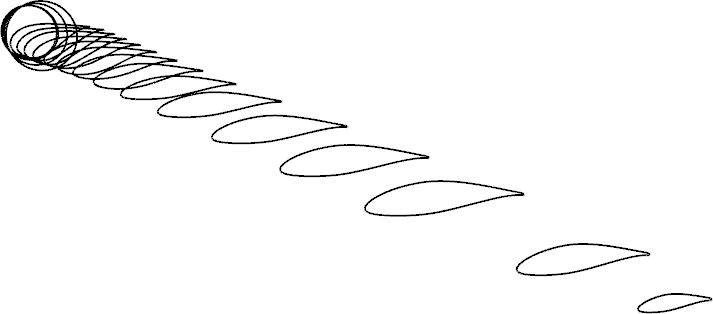
\includegraphics[width=.4\textwidth]{figs/airfoils}
    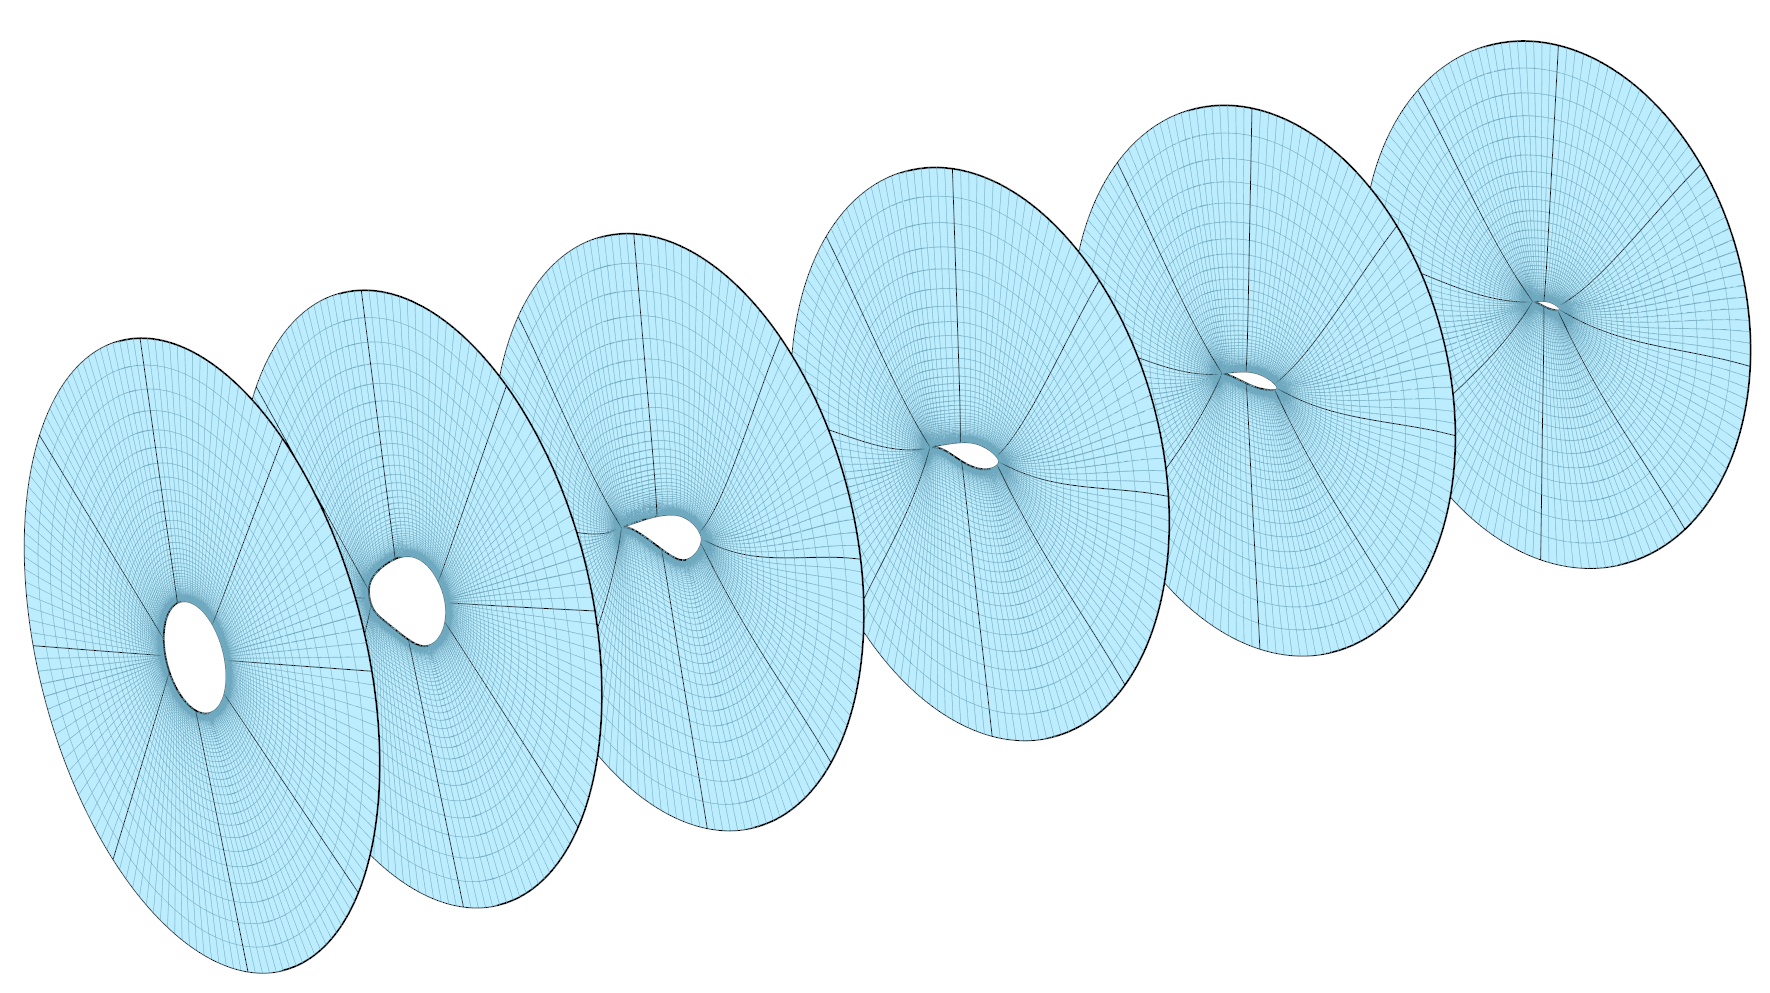
\includegraphics[width=.5\textwidth]{figs/crossecs2}
  \end{center}
  \caption{Airfoil cross-sections of an NREL 5MW reference wind turbine blade.}
  \label{fig:airfoils}
\end{figure}

\section{Impact}
\label{sec:impact}

Isogeometric analysis was introduced in 2005 \cite{hughes2005iac} for applying native B-spline basis functions for both the geometry and finite element solution.
One of the limiting factors of this endeavor has been that there have been sparse support for high quality B-spline mesh generation.
Traditional meshing tools used for finite element technologies typically produce Lagrangian piecewise linear simplex such as tetrahedrons.
Commercial software typically allow the user to create low-quality geometries containing gaps, overlaps and non-matching interfaces.
These are often referred to as ``dirty'' geometries by the industry, and while it is possible to create analysis suitable meshes, the process is currently tedious and time-consuming.

We hope that by this package allows researchers and engineers, especially in the isogeometric community, to consider more complex geometries.

While the package is a library and does not contain a dedicated graphical user interface (GUI), one should be able to create a CAD interface on top of it.
We note that of particular interest is FreeCAD, which is an open source CAD software and supports python plugins.
It would not be unreasonable to see a FreeCAD plugin of Splipy that would greatly increase its utility and user-friendliness.

% \textbf{This is the main section of the article and the reviewers weight the description here appropriately}
% \begin{itemize}
%   \item Indicate in what way new research questions can be pursued as a result of the software (if any).
%   \item Indicate in what way, and to what extent, the pursuit of existing research questions is improved (if so).
%   \item Indicate in what way the software has changed the daily practice of its users (if so).
%   \item Indicate how widespread the use of the software is within and outside the intended user group.
%   \item Indicate in what way the software is used in commercial settings and/or how it led to the creation of spin-off companies (if so).
% \end{itemize}

\section{Conclusions}
\label{sec:conclusion}

Splipy is a python programming library which empowers users to work with B-spline and NURBS representations of geometries.
It will lower the barrier of entry to create complex geometric shapes.
It allows for fine-grained control over parametrizations to ensure high-quality meshes which are tailored specifically for analysis.

\section*{Acknowledgments}
\label{}

The authors gratefully acknowledge the the financial support from the Norwegian Research Council and the FME NOWITECH (www.nowitech.no). They also acknowledge the support from the Norwegian University of Science and Technology.

%% The Appendices part is started with the command \appendix;
%% appendix sections are then done as normal sections
%% \appendix

%% \section{}
%% \label{}

%% References:
%% If you have bibdatabase file and want bibtex to generate the
%% bibitems, please use
%%
\bibliographystyle{elsarticle-num}{}
\bibliography{references}

%% else use the following coding to input the bibitems directly in the
%% TeX file.

%% \begin{thebibliography}{00}

%% \bibitem{label}
%% Text of bibliographic item

%% \bibitem{}

%% \end{thebibliography}

% \section*{Required Metadata}
% \label{}

\section*{Current code version}
\label{}

% Ancillary data table required for subversion of the codebase. Kindly replace examples in right column with the correct information about your current code, and leave the left column as it is.

\begin{table}[!h]
\begin{tabular}{|l|p{5.5cm}|p{7.5cm}|}
\hline
\textbf{Nr.} & \textbf{Code metadata description} & \textbf{Please fill in this column} \\
\hline
C1 & Current code version & 1.3 \\
\hline
C2 & Permanent link to code/repository used for this code version & $https://github.com/sintefmath/splipy$ \\
\hline
C3 & Legal Code License   & GNU General Public License v3.0  \\
\hline
C4 & Code versioning system used & git \\
\hline
C5 & Software code languages, tools, and services used & python \\
\hline
C6 & Compilation requirements, operating environments & numpy $\geq$ 1.15, scipy $\geq$ 1.2 \\
\hline
C7 & If available Link to developer documentation/manual & $https://sintefmath.github.io/splipy/$ \\
\hline
C8 & Support email for questions & Kjetil.Johannessen@sintef.no \\
\hline
\end{tabular}
\caption{Code metadata (mandatory)}
\label{}
\end{table}

% \section*{Current executable software version}
% \label{}
%
% Ancillary data table required for sub version of the executable software: (x.1, x.2 etc.) kindly replace examples in right column with the correct information about your executables, and leave the left column as it is.
%

\end{document}
\endinput
%%
%% End of file `SoftwareX_article_template.tex'.
